\documentclass[border=0.125cm]{standalone}
\usepackage{tikz}
\usepackage{pgfplots}
\usepackage{graphicx}

\usetikzlibrary{decorations.pathmorphing}
\pgfplotsset{compat=newest}
\usetikzlibrary{shapes.geometric,arrows,fit,matrix,positioning}
\tikzset{main node/.style={circle,fill=black!20,draw,minimum size=3.5mm,inner sep=0pt},
         every node/.style={circle,fill=black,draw,minimum size=1mm,inner sep=0pt,label distance=-1mm},
         subtree/.style={isosceles triangle,fill=black!20,draw,minimum size=5mm,inner sep=0pt,shape border rotate=90},
         edge label/.style = {rectangle,draw=none,fill=none},
         blank edge/.style={edge from parent/.style={draw=none}},
         norm edge/.style={edge from parent/.style={black,thin,draw}},
}
\begin{document}
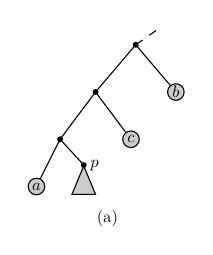
\begin{tikzpicture}[-,>=stealth', 
level 1/.style={sibling distance = 17mm},
level distance = 1cm, 
scale=0.6,
transform shape]
% \draw[help lines] (-2,2) grid (15,-15);
\node (0) {}
    child{
        [sibling distance = 15mm] node (1) {}
            child{
                [sibling distance = 10mm] node (2) {}
                    child{
                        node [main node] (3) {$a$}
                    }
                    child[edge from parent path = {(\tikzparentnode) -- (\tikzchildnode.north)}]{
                        node [subtree] (4) {}
                    }
            }
            child{
                node [main node] (5) {$c$}
            }
    }
    child{
        node [main node] (6) {$b$}
    }
;
\node [edge label, xshift = -6mm, below=35mm, align=flush center] at (0){
        {(a)}};
\node at (4.north){};        
\node[edge label,above right = 2mm and 0 mm of 4] {$p$};     
\draw[dashed] (0,0) -- (0.5,0.35);   
\end{tikzpicture}
~~~~~
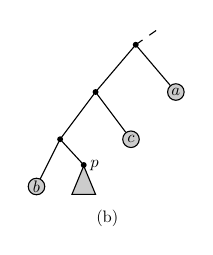
\begin{tikzpicture}[-,>=stealth', 
level 1/.style={sibling distance = 17mm},
level distance = 1cm, 
scale=0.6,
transform shape]
% \draw[help lines] (-2,0) grid (15,-15);
\node (0) {}
    child{
        [sibling distance = 15mm] node (1) {}
            child{
                [sibling distance = 10mm] node (2) {}
                    child{
                        node [main node] (3) {$b$}
                    }
                    child[edge from parent path = {(\tikzparentnode) -- (\tikzchildnode.north)}]{
                        node [subtree] (4) {}
                    }
            }
            child{
                node [main node] (5) {$c$}
            }
    }
    child{
        node [main node] (6) {$a$}
    }
;
\node [edge label, xshift = -6mm, below=35mm, align=flush center] at (0){
        {(b)}};
\node at (4.north){};        
\node[edge label,above right = 2mm and 0 mm of 4] {$p$};       
\draw[dashed] (0,0) -- (0.5,0.35);    
\end{tikzpicture}

\end{document}



















